\subsection{Vision-Language Models for Document Understanding}
\subsubsection{Foundational Vision-Language Models for Document Understanding}
The development of Vision-Language Models (VLM) has propelled visual document understanding from single-modality analysis toward a unified multimodal modeling paradigm. By jointly modeling visual content, textual semantics, and spatial layout information, VLMs enable systems to gain a deeper understanding of document structures and their semantic relationships. Building on this capability, visual document understanding has gradually evolved into a general intelligent system characterized by structure awareness, cross-modal reasoning, and document-level understanding. The following sections introduce the evolution of VLMs across four key dimensions.

\paragraph{Foundational Period of Visually-Rich Document Understanding}
Early research established the technical foundations for document image classification and cross-modal retrieval.
Deep multimodal learning for cross-modal retrieval: One model for all tasks \cite{wei2020deep} proposed a "unified model" approach, encoding vision and text into the same retrievable representation space to simultaneously support bidirectional image-text retrieval and unimodal retrieval within a single model.
Entering the pre-training era, Layoutxlm: Multimodal pre-training for multilingual visually-rich document understanding \cite{xu2021layoutxlm} introduced a multimodal pre-training model for multilingual, visually-rich documents, integrating text, layout, and visual information into a unified multilingual pre-training framework.
VinVL: Revisiting Visual Representations in Vision-Language Models \cite{zhang2021vinvl} systematically investigated the role of "visual features themselves" in multimodal tasks, proving that high-quality visual encoding is a key factor in enhancing VLM performance.
CLIP-Adapter: Better Vision-Language Models with Feature Adapters \cite{gao2021clipadapter} proposed an efficient way to adapt CLIP without compromising its pre-training capabilities by adding lightweight ``adapter'' modules in the feature space to improve performance on few-shot and downstream tasks.
In 2022, the research community began focusing on constructing generalized document processors.
FLAVA: A Foundational Language And Vision Alignment Model \cite{singh2022flava} presented a foundational model for general vision-language understanding, proposing the use of both image-text pairs and unimodal data for pre-training under a unified Transformer architecture to balance cross-modal alignment and unimodal understanding.
Unifying Vision, Text, and Layout for Universal Document Processing \cite{li2022udop} proposed the UDOP framework, which models visual appearance, textual content, and spatial layout in documents as a unified sequence-to-sequence generative task, supporting various document understanding and generation tasks through an instructional prompt mechanism.
Unified Pretraining Framework for Document Understanding \cite{wang2022unified} proposed a unified document pre-training framework that performs large-scale pre-training by multimodally encoding semantic regions in documents and combining multiple self-supervised learning objectives, thereby improving model transfer and generalization across different document understanding tasks.
Bi-VLDoc: Bidirectional Vision-Language Modeling for Visually-Rich Document Understanding \cite{yang2022bivldoc} designed a bidirectional vision-language supervision mechanism, enabling the model to predict language from vision and vice versa, strengthening cross-modal alignment and semantic interaction.
Multimodal pre-training based on graph attention network for document understanding \cite{liu2022gatdoc} explicitly modeled document structure as a graph and performed multimodal pre-training based on Graph Attention Networks, allowing the model to better capture contextual dependencies driven by layout relationships.
CM3: A Causal Masked Multimodal Model of the Internet \cite{ai2022cm3} adopted a generative multimodal pre-training strategy using causal masking, modeling text and image tokens in a unified sequence to provide the model with both multimodal understanding and generation capabilities.
NLX-GPT: A Model for Natural Language Explanations in Vision and Vision-Language Tasks \cite{kayser2022nlxgpt} introduced a unified model for simultaneously predicting answers and generating natural language explanations in vision and vision-language tasks.
Furthermore, Vision and natural language for metadata extraction from scientific PDF documents: a multimodal approach \cite{li2022pdfmeta} proposed a multimodal method merging visual layout and textual semantics to automatically extract structured metadata from scientific PDF documents.
I2MVFormer: Large Language Model Generated Multi-View Document Supervision for Zero-Shot Image Classification \cite{zhao2022i2mvformer} utilized Large Language Models to generate multi-view textual descriptions as supervision signals, enhancing semantic modeling in zero-shot image and document classification.

\paragraph{The Rise of VLM and Advancements in High-Resolution Perception}
With the integration of Large Language Models (LLMs), document understanding entered an instruction-driven phase.
PaLM-E: An Embodied Multimodal Language Model \cite{driess2023palme} proposed an embodied multimodal language model, enabling language models to directly process inputs from various sensors and achieve integrated modeling of visual, linguistic, and embodied reasoning tasks.
MiniGPT-4: Enhancing Vision-Language Understanding with Advanced Large Language Models \cite{zhu2023minigpt4} explored how advanced LLMs can improve vision-language understanding by aligning features from a frozen visual encoder with a powerful pre-trained LLM (such as Vicuna) using only a single projection layer, significantly enhancing visual description and text generation while retaining visual and linguistic capabilities.
PaLI-X: On Scaling up a Multilingual Vision and Language Model \cite{chen2023palix} introduced a large-scale multilingual VLM that achieved significant performance gains in multilingual image captioning, visual question answering, document understanding, and few-shot learning by scaling component sizes and task diversity.
mPLUG-PaperOwl: Scientific Diagram Analysis with the Multimodal Large Language Model \cite{ye2023paperowl} focused on enhancing the understanding and analysis of scientific diagrams by general multimodal LLMs, significantly outperforming existing models in multimodal diagram description, analysis, and outline recommendation, demonstrating powerful capabilities in deep scientific diagram parsing and opening new directions for academic content generation.
Additionally, UniDoc: A Universal Large Multimodal Model for Simultaneous Text Detection, Recognition, Spotting and Understanding \cite{li2023unidoc} proposed a unified multimodal large model framework capable of end-to-end text detection, recognition, spotting, and semantic understanding within a single model---a holistic capability previously unavailable in similar methods.
Between 2023 and 2024, high-resolution processing became the core focus.
Monkey: Image Resolution and Text Label Are Important Things for Large Multimodal Models \cite{li2024monkey} systematically studied the impact of image resolution and text label quality on MLLM performance, noting that in document understanding and text-dense scenarios, resolution improvements often yield more direct and significant gains than structural changes, as high-resolution input markedly improves the perception of fine-grained text, symbols, and layout structures.
TextMonkey: An OCR-Free Large Multimodal Model for Understanding Documents \cite{li2024textmonkey}, building on the analysis of Monkey, proposed an end-to-end OCR-free document understanding model that performs joint visual and semantic modeling directly from high-resolution document images.
Qwen2-VL: Enhancing Vision-Language Model's Perception of the World at Any Resolution \cite{wang2024qwen2vl} addressed the instability of VLM perception under different resolution conditions by proposing a unified modeling framework supporting arbitrary resolution inputs.
DocKylin: A Large Multimodal Model for Visual Document Understanding with Efficient Visual Slimming \cite{liu2024dockylin} focused on the computational overhead brought by high-resolution inputs, proposing an efficient visual slimming strategy that maintains document understanding performance while significantly reducing the number of visual tokens.
DocPedia: Unleashing the Power of Large Multimodal Model in the Frequency Domain for Versatile Document Understanding \cite{zhao2023docpedia} explored the potential value of frequency-domain information in visual document understanding, breaking the traditional paradigm that relies almost exclusively on spatial-domain features by merging frequency-domain representations with spatial features to better capture repetitive textures and structural patterns.
Meanwhile, Vary: Scaling up the Vision Vocabulary for Large Vision-Language Models \cite{huang2023vary} argued from the perspective of visual representation discretization that existing VLMs face expression bottlenecks in visual vocabulary scale, requiring a systematic expansion of the visual vocabulary to allow the model to express complex image content with finer-grained visual tokens.
DocLLM: A layout-aware generative language model for multimodal document understanding \cite{wang2024docllm} proposed an explicitly layout-aware generative language model that directly integrates spatial structure information into the language generation process, ensuring generated results align with the document's structural logic and semantic organization.
mPLUG-DocOwl 1.5: Unified Structure Learning for OCR-free Document Understanding \cite{hu2024mplugdocowl15} further strengthened structure learning capabilities under an OCR-free framework, proposing a unified structure modeling mechanism to capture relationships between text, layout, and visual cues.
For chart-centric document scenarios, TinyChart-3B \cite{zhang2024tinychart} demonstrated that specialized lightweight MLLMs can achieve strong structural and numerical reasoning by combining visual token merging with Program-of-Thoughts learning, thereby attaining high chart understanding performance with only 3B parameters.
Qwen-VL: A Versatile Vision-Language Model for Understanding, Localization, Text Reading, and Beyond \cite{bai2023qwenvl} introduced a highly versatile VLM framework supporting image understanding, region localization, text reading, and cross-modal reasoning, performing exceptionally well in text-dense and complex layout scenarios.
Furthermore, document understanding for small models has gained attention.
PaLI-3 Vision Language Models: Smaller, Faster, Stronger \cite{chen2023pali3} achieved stronger multimodal understanding at a smaller model scale through architectural design and training strategy optimization, greatly expanding application scenarios.
Small Language Model Meets with Reinforced Vision Vocabulary \cite{li2024slmrvv} explored the potential of Small Language Models (SLMs) in multimodal contexts, proposing to compensate for limited model scale by reinforcing the vision vocabulary. By enhancing the expressive power on the visual side, small models significantly improved their performance in document understanding and visual reasoning, approaching the level of large models in certain scenarios.
To optimize alignment, Enhancing Visual Document Understanding with Contrastive Learning in Large Visual-Language Models \cite{wu2024contrastivedoc} introduced contrastive learning objectives to enhance the alignment between visual and textual representations, thereby mitigating semantic mismatch issues in complex documents.
Read and Think: An Efficient Step-wise Multimodal Language Model for Document Understanding and Reasoning \cite{lu2024readthink} proposed a stepwise multimodal reasoning framework that decomposes document understanding into sequential reading and reasoning stages, improving the model's ability to handle long documents and complex questions while maintaining computational efficiency.
Gemini: A Family of Highly Capable Multimodal Models \cite{team2023gemini} introduced a family of unified multimodal large models covering text, images, audio, and video. In visual document understanding scenarios, Gemini demonstrated powerful cross-modal reasoning and contextual integration capabilities.
VisionLLM v2: An End-to-End Generalist Multimodal Large Language Model for Hundreds of Vision-Language Tasks \cite{wang2024visionllmv2} unified a vast array of vision-language tasks in an end-to-end manner, emphasizing versatility and scalability. In document understanding, it showed stable cross-task generalization, representing the trend toward general-purpose multimodal models.
EVLM: An Efficient Vision-Language Model for Visual Understanding \cite{li2024evlm} optimized visual encoding and cross-modal fusion modules from a holistic system efficiency perspective, balancing performance and computational cost across various tasks.
3MVRD: Multimodal Multi-task Multi-teacher Visually-Rich Form Document Understanding \cite{zhang2024mmvrd} proposed a multimodal, multi-task, multi-teacher distillation framework for joint modeling of visually-rich documents. Through collaborative guidance from multiple teachers, the model showed stronger generalization in multi-task scenarios, reflecting the effectiveness of knowledge transfer in document understanding.
A LayoutLMv3-Based Model for Enhanced Relation Extraction in Visually-Rich Documents \cite{li2024layoutlmv3re} reinforced relation extraction in visually-rich documents based on LayoutLMv3, highlighting the role of layout information in structured semantic modeling and proving that explicit layout modeling can effectively improve the accuracy of entity relationship understanding.
\begin{figure*}[t]
\centering
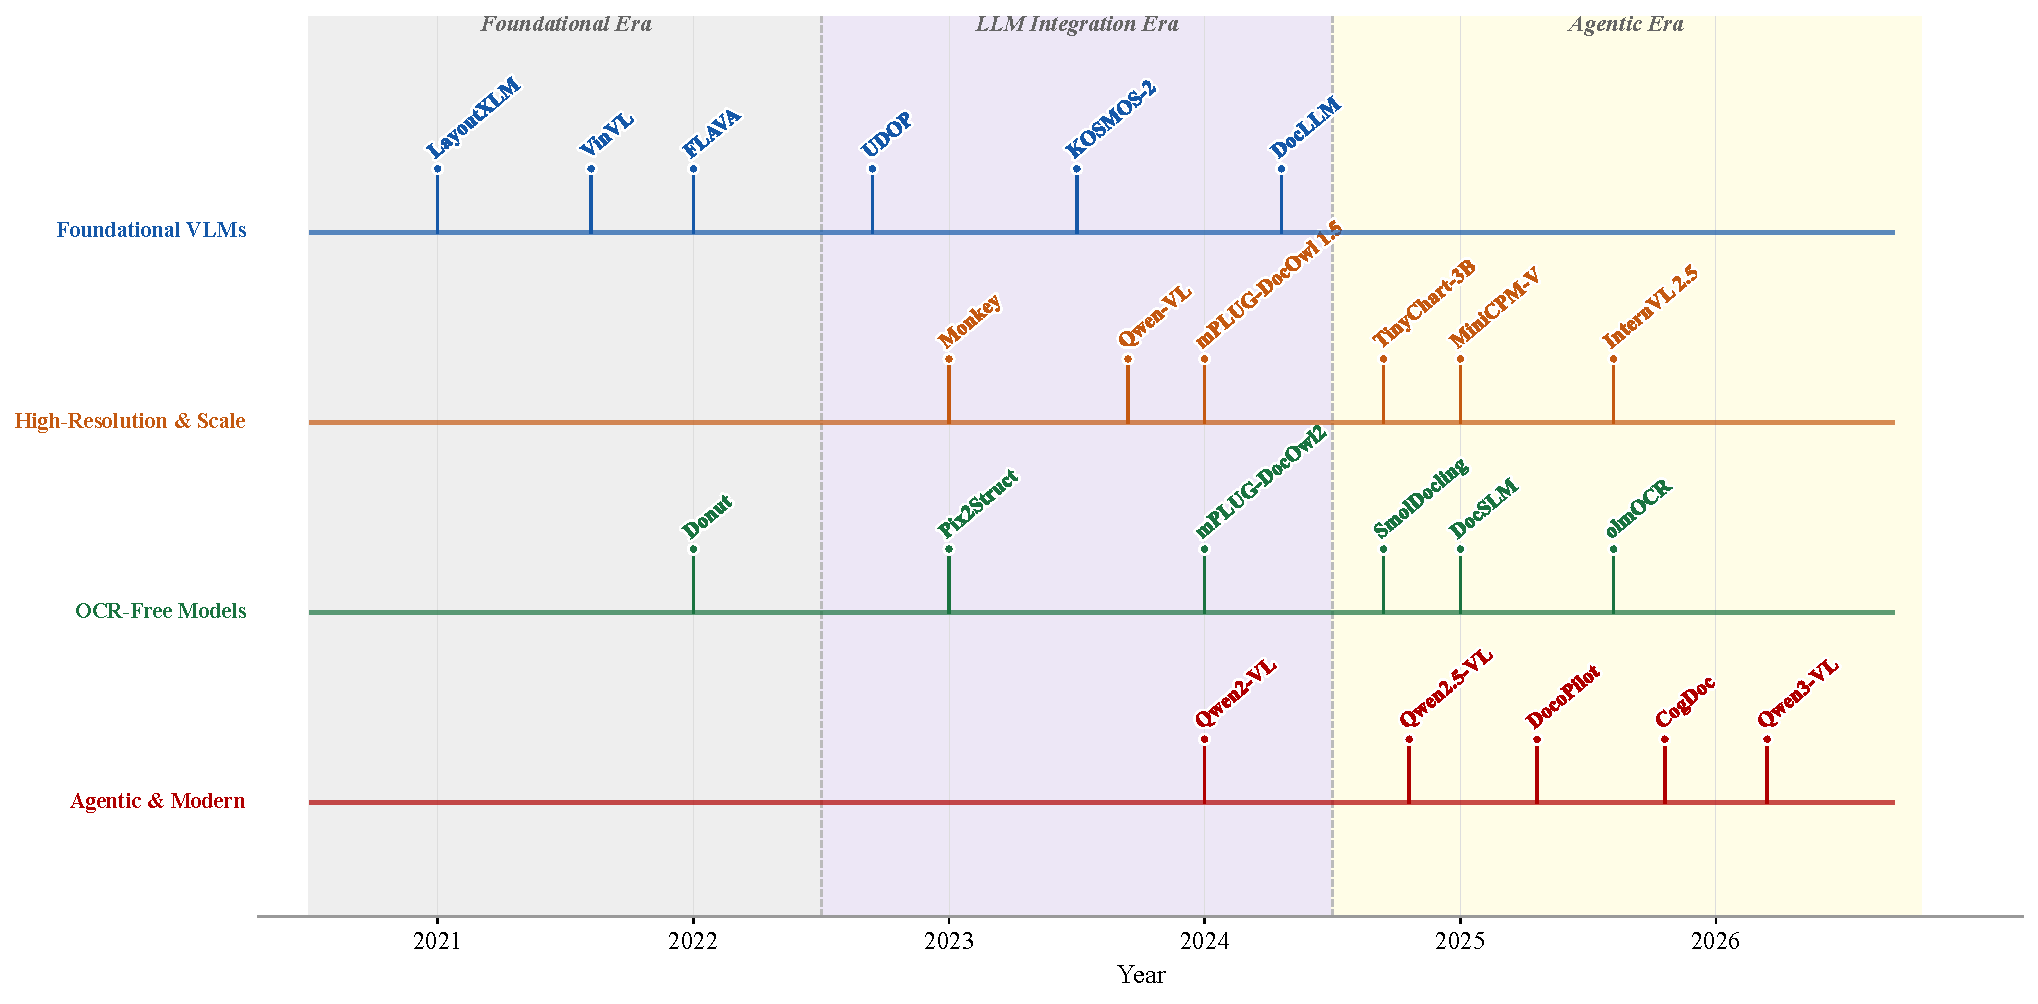
\includegraphics[
    width=0.95\textwidth,
    trim=0cm 0cm 0cm 0cm,
    clip
]{figs_by_qixingyu/fig07.pdf}
\caption{Evolution of vision-language models for document understanding (2021--2026)---organized into four development tracks: foundational vision-language models, high-resolution and scaled architectures, OCR-free models, and agentic systems for complex document reasoning.}
\label{fig:vlm_evolution}
\end{figure*}

\paragraph{The Evolution of OCR-free and Multi-page Context}
Moving away from traditional OCR dependency and handling long documents are key steps toward the practicality of VRDU. Traditional document understanding methods usually rely on Optical Character Recognition (OCR) systems to convert document images into text before performing semantic analysis. However, this process disconnects "text recognition" and "document understanding" into two independent steps; if OCR makes an error or structural information is lost, subsequent models struggle to recover the original semantics. OCR-free models utilize joint vision-language modeling, taking raw document images as direct input, using visual encoders to extract features, and using structures like Transformers to generate text or structured results in an end-to-end fashion. Such an approach allows the model to implicitly learn character and semantic information without explicitly calling an OCR system. This unified modeling avoids OCR error propagation and more completely preserves the layout and visual context, showing stronger robustness and generalization in complex layouts, multi-page documents, and cross-modal understanding tasks.
OCR-free Document Understanding Transformer (Donut) \cite{kim2022donut} was an end-to-end document understanding model that did not rely on OCR systems. Based on a Transformer encoder-decoder structure, it generates structured text output directly from raw document images, avoiding error propagation in traditional OCR pipelines. Experimental results show that Donut achieves competitive performance across various tasks while significantly simplifying the document processing workflow.
Pix2Struct \cite{lee2023pix2struct} proposed an OCR-free VLM based on screenshot parsing pre-training, capable of generating structured text representations directly from raw images using a Transformer encoder-decoder architecture to achieve unified vision-language understanding.
mPLUG-DocOwl: Modularized Multimodal Large Language Model for Document Understanding \cite{ye2023docowl} introduced a modularized MLLM for OCR-free document understanding to address the issue of existing models ignoring fine-grained visual features in complex scenarios, demonstrating stronger cross-task generalization even without specific fine-tuning.
mPLUG-DocOwl2: High-resolution Compressing for OCR-free Multi-page Document Understanding \cite{ye2024docowl2} proposed an efficient visual compression and structural modeling method for multi-page documents to address the computational and contextual bottlenecks in OCR-free scenarios. This model compresses and aggregates cross-page visual information while maintaining high-resolution perception, significantly reducing visual token counts and supporting long-document modeling.
DeepSeek-VL2: Mixture-of-Experts Vision-Language Models for Advanced Multimodal Understanding \cite{deepseek2024vl2} adopted the Mixture-of-Experts (MoE) architecture in VLMs, significantly improving parameter efficiency through an expert routing mechanism that dynamically activates sub-models for different types of visual and semantic inputs.
Regarding complex document parsing, MinerU2.5 \cite{liu2025mineru25} proposed an efficient high-resolution document parsing framework. It employs a coarse-to-fine two-stage parsing strategy to address computational bottlenecks: the first stage performs global layout analysis on downsampled images to identify structural elements, while the second stage crops key regions based on the global layout.
POINTS-Reader: Distillation-Free Adaptation of Vision-Language Models for Document Conversion \cite{wang2025pointsreader} proposed a distillation-free adaptation framework focusing on the lack of high-quality annotated data in complex document conversion tasks.
PDF-WuKong: A Large Multimodal Model for Efficient Long PDF Reading with End-to-End Sparse Sampling \cite{li2024pdfwukong} addressed the challenges of merging large-scale visual and textual information in long PDF documents by selecting paragraphs or charts most relevant to user queries, avoiding redundant computation of the entire document.
LongFin: A Multimodal Document Understanding Model for Long Financial Domain Documents \cite{chen2024longfin} introduced a model specifically designed for multimodal understanding of long financial documents, breaking the maximum length limits of traditional models to accommodate multi-page, long-content industrial financial documents.
Furthermore, H2OVL-Mississippi Vision Language Models Technical Report \cite{h2ovl2024mississippi} introduced a suite of small VLMs aimed at meeting the needs for efficient, lightweight document processing in privacy-sensitive and on-device scenarios.
FILA: Fine-Grained Vision Language Models \cite{liu2024fila} focused on the fine-grained visual understanding capabilities of MLLMs when processing high-resolution images, providing a solution to the object truncation and semantic fragmentation issues caused by dynamic cropping and re-encoding.
Expanding Performance Boundaries of Open-Source Multimodal Models with Model, Data, and Test-Time Scaling \cite{chen2024internvl25} presented the InternVL 2.5 series, systematically studying the impact of model scale, data quality, and test-time strategies on MLLM performance and providing a deep analysis of each factor's contribution to multimodal understanding.
Additionally, Multimodal Adaptive Inference for Document Image Classification with Anytime Early Exiting \cite{sun2024anytime} proposed a multimodal adaptive inference framework to balance efficiency and performance in VRDU tasks by embedding multi-layer early exiting mechanisms within the base model.

\paragraph{Modern Document Understanding Evolution}
The years 2025 and 2026 witnessed an explosion of ultra-lightweight models.
DocSLM: A Small Vision-Language Model for Long Multimodal Document Understanding \cite{wang2025docslm} proposed an efficient small VLM to address the computational and memory bottlenecks of large-scale VLMs in long document understanding and edge deployment, achieving or exceeding state-of-the-art performance with significantly fewer parameters.
SmolDocling: An ultra-compact vision-language model for end-to-end multimodal document conversion \cite{kim2025smoldocling} focused on end-to-end multimodal document conversion, proposing an extremely compact VLM that processes complete pages within a single network and expresses all elements and their positions through a universal tagging format called DocTags.
Specific applications and vertical domain research include Baseer: A Vision-Language Model for Arabic Document-to-Markdown OCR \cite{albaseer2025baseer}, which designed a specialized VLM for the unique challenges of Arabic OCR and fine-tuned it on a mixed dataset of synthetic and real documents to accurately convert Arabic documents into structured Markdown.
IndoColSmol: Lightweight Vision-Language Models for Multimodal Indonesian Document Search \cite{rahman2025indocolsmol} proposed two lightweight vision-language retrieval models focused on multimodal retrieval tasks for Indonesian documents.
Semantic Document Derendering: SVG Reconstruction via Vision-Language Modeling \cite{kim2025derendering} introduced a multimodal-based vectorization tool to parse complex document images into editable vector formats.
Qwen2.5-VL Technical Report \cite{bai2025qwen25vl} established performance benchmarks for unified vision-language understanding, localization, and text reading.
Qwen3-VL Technical Report \cite{bai2025qwen3vl} further expanded model capacity and reasoning capabilities, enhancing cross-modal task generalization and fine-grained perception.
Finally, document-level strategy research includes Docopilot: Improving Multimodal Models for Document-Level Understanding \cite{duan2025docopilot}, which addressed the shortcomings of MLLMs in multi-page document-level tasks by proposing a native document-level multimodal large model framework to replace retrieval-augmented generation methods.
Nayana: A Foundation for Document-Centric Vision-Language Models via Multi-Task \cite{kolavi2025nayana} aimed to build a multi-task, multimodal, and multilingual foundational resource and training framework, significantly expanding the potential of VLMs in global document understanding scenarios.
PP-DocBee2: Improved Baselines with Efficient Data for Multimodal Document Understanding \cite{du2025docbee2} proposed a set of foundational enhancement strategies for end-to-end document image understanding.
Interpret, prune and distill Donut: towards lightweight VLMs for VQA on document \cite{zhou2025donutdistill} focused on compressing generative VLMs like Donut into lightweight versions using interpretation, pruning, and distillation for efficient Document VQA.
LoRA-Contextualizing Adaptation of Large Multimodal Models for Long Document Understanding \cite{li2025loracontext} introduced LoRA structures to VLMs, allowing the model to serve as an efficient base for self-visual retrieval-augmented generation frameworks while adapting to long-document tasks through fine-grained parameter adjustments.
SCoPE VLM: Selective Context Processing for Efficient Document Navigation in Vision-Language Models \cite{wang2025scopevlm} proposed a strategy called "Chain of Scroll" for selective and recursive navigation in long documents to avoid the high memory consumption of processing full pages at once.
Entering 2026, A Hybrid Architecture for Multi-Stage Claim Document Understanding: Combining Vision-Language Models and Machine Learning for Real-Time Processing \cite{patel2026claim} proposed a multi-stage hybrid architecture for the automated processing of medical and insurance claim documents, designing an end-to-end pipeline to handle challenges like mixed layouts, handwriting, and diverse languages in scanned or photographed documents.

\subsubsection{Multimodal RAG}
Building on the success of text RAG in pure text QA, researchers began extending the retrieval-augmented paradigm to Visual Document Question Answering (DocQA/DocVQA), forming an early multimodal transition path centered on OCR/structural parsing + text retrieval. This stage generally assumed that document semantics primarily stem from text, using OCR to convert visual documents into text and layout structures before expanding retrieval and generation capabilities. PDF-MVQA \cite{ding2024mvqa} noted the bias of existing benchmarks toward single-page sparse text and constructed a multi-page visually-rich document QA dataset, proposing a joint coarse-to-fine retrieval framework for cross-page localization. CREAM \cite{zhang2024cream} introduced a coarse-to-fine retrieval pipeline and merged multi-page visual encoding to address evidence sparsity and retrieval efficiency in long contexts. DocLLM \cite{wang2024docllm} mitigated the neglect of text-layout relationships in traditional VLMs by explicitly modeling spatial layout, improving the stability of generative DocQA. ViTLP \cite{mao2024visually} jointly modeled text and layout during pre-training, enabling the model to handle long documents without relying on ultra-long contexts. Overall, this series of work established the OCR + text RAG paradigm centered on textual evidence with layout and vision as aids, providing a key transition for subsequent OCR-free and deeper multimodal fusion methods.

As the "OCR + text retrieval" method exposed issues of structural and visual information loss in visually-rich documents, research shifted toward OCR-free visual retrieval paradigms, completing retrieval and alignment directly in the original visual space of the document. ColPali \cite{faysse2024colpali} proposed a page-level OCR-free document retrieval method, using VLMs to generate multi-vector page representations and achieving multi-granularity matching between queries and pages through a late-interaction mechanism, significantly improving retrieval robustness for complex layouts while introducing the ViDoRe benchmark to systematically evaluate OCR-free retrieval. Document Screenshot Embedding \cite{ma2024unifying} further used document screenshots as a unified retrieval input, jointly encoding text, images, and layout into dense vectors through large VLMs, allowing a single retrieval system to adapt to various document forms.

After OCR-free page retrieval began solving visual structure fidelity and cross-modal alignment, multimodal RAG research moved toward a stage centered on multi-page, multi-document, multimodal evidence fusion and reasoning consistency. The focus shifted from "whether relevant pages can be retrieved" to "how to organize, align, and verify scattered evidence in complex document collections." Representative works like VisRAG \cite{yu2024visrag} and VDocRAG \cite{tanaka2025vdocrag} were pioneers in introducing VLMs to the retrieval stage, using the overall visual representation of a page or document to drive generation, laying the foundation for cross-chart and cross-layout QA. M3DocRAG \cite{cho2024m3docrag} systematically proposed multi-page, multi-document, multimodal DocQA tasks and significantly improved cross-document evidence coverage by integrating visual cues into the RAG workflow. Subsequent research deepened at the level of evidence organization and reasoning: CMRAG \cite{chen2025cmrag} mitigated unimodal bias through dual-channel retrieval of text and images; RegionRAG \cite{li2025regionrag} lowered retrieval granularity to the region level to reduce visual noise; MHier-RAG \cite{gong2025mhier} integrated fragmented cross-page evidence with hierarchical indexing; MoLoRAG \cite{wu2025molorag} and QCG-RAG \cite{wu2025query} introduced logic-aware and query-driven graph structures to enhance multi-hop reasoning; and HKRAG \cite{tong2025hkrag} improved answer completeness through holistic modeling of salient knowledge and fine-grained details. Furthermore, Luminirag \cite{martis2024luminirag} and MMGraphRAG \cite{wan2025mmgraphrag} unified vision and text into graph structures for structured cross-modal retrieval and interpretable reasoning. AutoThinkRAG \cite{autothinkrag} further advanced this line by introducing a query-complexity-aware router that dynamically allocates retrieval and reasoning paths, enabling more efficient multimodal DocQA under long and information-dense document settings. In addition, AutoThinkRAG proposed a decoupled perception-and-reasoning paradigm, where a lightweight VLM first translates query-relevant visual evidence into textual descriptions and an LLM subsequently performs logical synthesis, alleviating the reasoning bottleneck of end-to-end VLMs. TableRAG \cite{yu2025tablerag} extended this to heterogeneous text-table documents, maintaining structural semantics through retrieval combined with programmatic execution. VisDoM \cite{suri2025visdom} and ViDoRAG \cite{wang2025vidorag} utilized multi-step or multi-agent reasoning to improve evidence combination across multiple documents. Finally, Look as You Think \cite{liu2025look} and RAG-Anything \cite{guo2025rag} advanced this line further from the perspectives of verifiable reasoning and unified knowledge representation, with the former using reinforcement learning to achieve precise attribution of reasoning steps and visual evidence, and the latter integrating all-modality knowledge with dual-graph structures. This stage marks the transition of multimodal RAG from "retrieval-augmented generation" to a systematic framework of "evidence orchestration, reasoning consistency, and verifiability," providing a more robust and interpretable path for real-world complex DocQA.

\subsubsection{Agentic Frameworks for Document QA}
In recent years, research on multi-document and long-document QA has shifted from static RAG to agentic reasoning frameworks with process modeling capabilities. Early work relied on concatenating document snippets as input to LLMs, which suffered from deficiencies in evidence integration, reasoning controllability, and hallucination suppression. CuriousLLM \cite{yang2025curiousllm}, based on Knowledge Graph Prompting (KGP) and graph traversal agents, introduced a curiosity-driven follow-up question generation mechanism. This allows the model to actively guide retrieval and expand evidence coverage, mitigating the loss of reasoning direction in multi-document QA while reducing the computational and latency overhead of the original KGP methods.
In visually-rich long document scenarios, simple text-level retrieval struggles to locate key evidence. DocLens \cite{zhu2025doclens} proposed a tool-enhanced multi-agent framework for long visual document understanding, achieving step-by-step focusing from the entire document to key pages and visual elements through explicit page-level zooming (Lens) and a sampling-judging mechanism, showing significant improvements over traditional long-context strategies.
From a more general RAG perspective, MA-RAG \cite{nguyen2025ma} pointed out that a single retrieval-generation process struggles with query ambiguity and evidence sparsity. It introduced a multi-agent system with a clear division of labor, decoupling question decomposition, retrieval control, evidence extraction, and answer synthesis through collaborative chain-of-thought communication to systematically improve multi-hop QA performance.
For collection-level retrieval and reasoning of visual documents, ViDoRAG \cite{wang2025vidorag} proposed a dynamic iterative reasoning agent. By using hybrid multimodal retrieval strategies and an exploration-reflection workflow, it strengthened joint reasoning of visual and textual evidence and provided the ViDoSeek benchmark to address the lack of evaluation for large-scale visual document collections.
Further targeting "research-level" complex queries, Doc-Researcher \cite{dong2025doc} unified multimodal document parsing, dynamic multi-granularity retrieval, and multi-agent reasoning into an end-to-end system, emphasizing evidence chain accumulation and cross-modal consistency, with systematic evaluation of multi-hop and multi-round capabilities via M4DocBench.
Parallel agent research also includes visual agents for interactive environments. CogAgent \cite{hong2024cogagent} built a VLM-based agent capable of understanding and navigating interfaces directly from high-resolution screen pixels, demonstrating the scalability of agentic visual understanding in non-document environments.
At the methodological level, HEAR \cite{chen2025hear} explicitly introduced agentic reasoning into the document understanding process, establishing coordination between information extraction and reasoning generation to organize multimodal evidence actively.
Finally, CogDoc \cite{xu2025cogdoc} proposed a unified coarse-to-fine thinking paradigm based on cognitive modeling. Through a two-stage coordination of fast localization and deep reasoning, combined with reinforcement learning for strategy optimization, it mitigates fine-grained semantic loss while maintaining scalability.

\begin{figure*}[t]
\centering
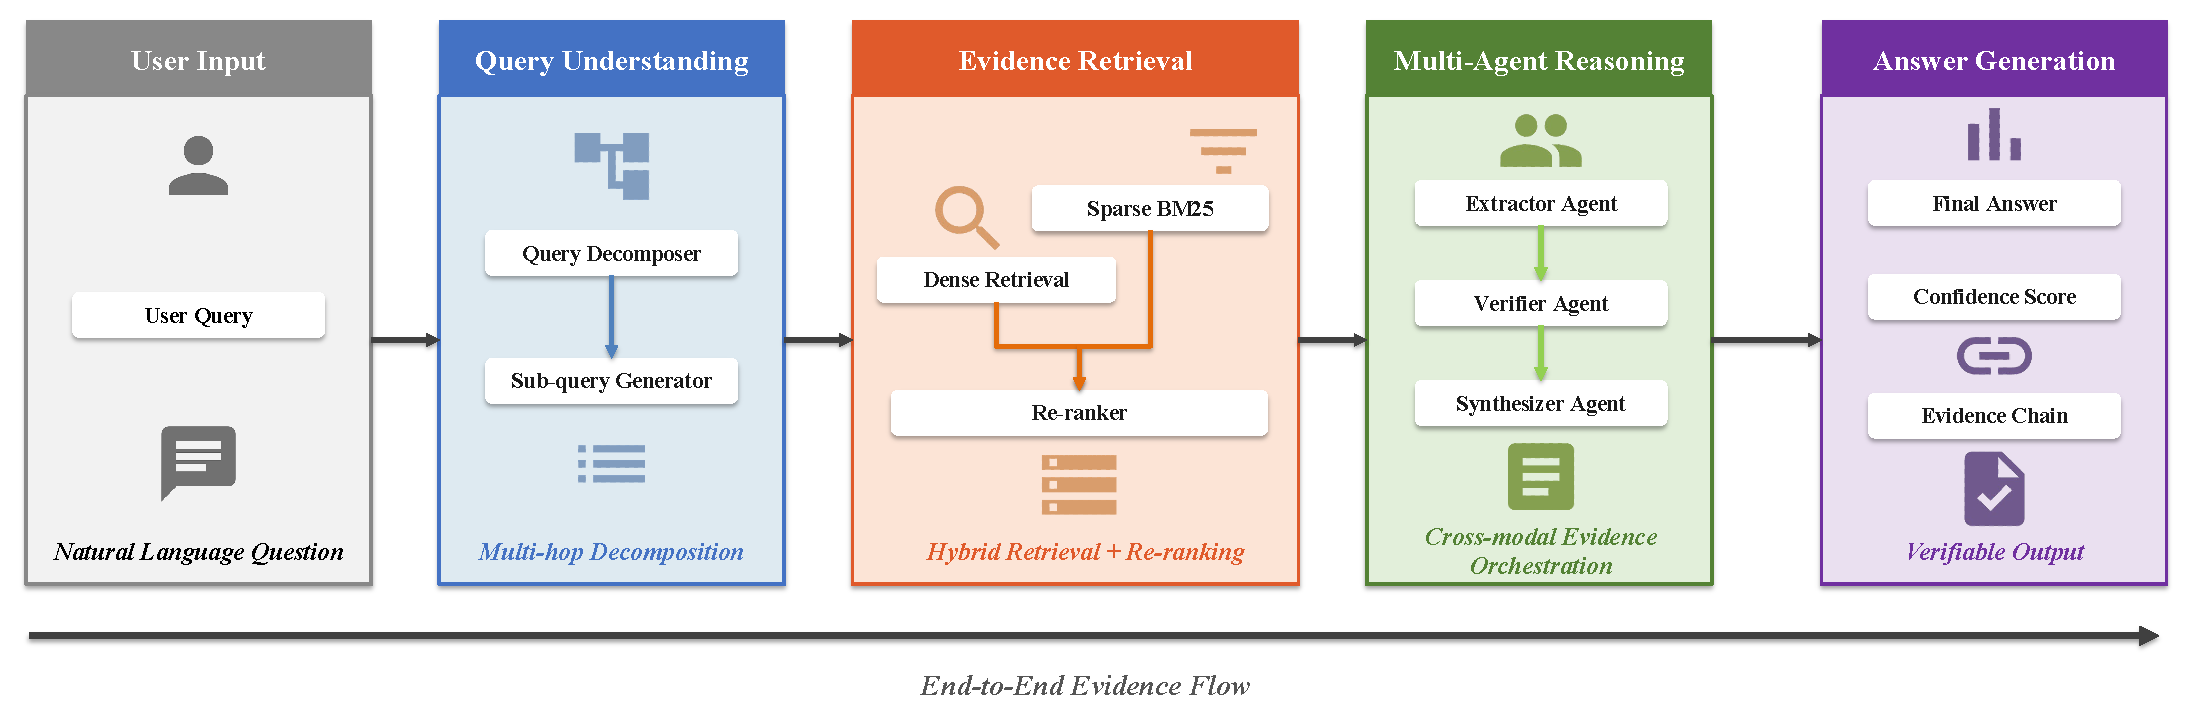
\includegraphics[
    width=0.95\textwidth,
    height=0.40\textheight,
    keepaspectratio,
    trim=0cm 0cm 0cm 0cm,
    clip
]{figs_by_qixingyu/fig08.pdf}
\caption{Agentic Document QA pipeline illustrating end-to-end evidence flow: a user natural language query passes through Query Understanding (multi-hop decomposition), Evidence Retrieval (hybrid dense and sparse retrieval with re-ranking), Multi-Agent Reasoning (extractor, verifier, and synthesizer agents for cross-modal evidence orchestration), and Answer Generation (producing a final answer with an evidence chain and confidence score).}
\label{fig:agent_docqa}
\end{figure*}